\documentclass[conference]{IEEEtran}

\usepackage{amsmath,amssymb,amsfonts}
\usepackage{array}
\usepackage{booktabs}
\usepackage{cite}
\usepackage{graphicx}
\usepackage{hyperref}
\usepackage{xcolor}

\newcolumntype{P}[1]{>{\raggedright\arraybackslash}p{#1}}
\graphicspath{{../../figures/}{../../../benchmarks/results/}{../../../benchmarks/angle_sweep_results/}}

\begin{document}

\title{Compute Practicality and Implementation Realism of the Wide View and Line Filters}

\author{\IEEEauthorblockN{J.C.\ Vaught}
\IEEEauthorblockA{Department of Computer Science and Engineering\\
University of South Carolina\\
Columbia, SC, USA}}

\maketitle

\begin{abstract}
The Wide View Filter (WVF) and Line Filter (LF) papers make strong claims about edge quality in aquatic and low-visibility scenes, but those claims only matter operationally if the implementation is practical on real hardware. This paper audits compute practicality rather than edge accuracy. Using the local repository implementation, exact 1001-threshold A100 benchmark reports, provisional WVF/LF scale-sweep logs, and a new 112-core defq parallelization path, we show that the current WVF/LF code is a CPU-only NumPy/SciPy implementation with nested per-pixel and per-orientation least-squares solves. The benchmark infrastructure is heterogeneous: classical filters and WVF/LF run on CPU, while the ML baselines use PyTorch and can move to CUDA when available. Exact BSDS500 and UDED runs on A100 hardware confirm that large-support Sobel remains competitive or better than the reproduced ML baselines under the current protocol, but they do not make WVF/LF operationally lightweight because WVF/LF was not benchmarked in the same GPU-backed path. The new defq parallelization reduces wall-clock time for sweeps by distributing independent tasks across up to 112 CPU workers, yet it does not change the underlying algorithmic cost of WVF/LF. The practical conclusion is narrow: the method is mathematically plausible, but the present implementation is still far from a lightweight baseline.
\end{abstract}

\begin{IEEEkeywords}
edge detection, compute practicality, runtime fairness, SLURM, NumPy, PyTorch, reproducibility
\end{IEEEkeywords}

\section{Introduction}
The compute question around WVF/LF is not whether the method can produce interesting gradients. It can. The question is whether the method can be treated as a practical baseline in the same sense as a classical derivative filter or a modern GPU-backed detector. That distinction matters because the source papers motivate the method for challenging aquatic and low-visibility scenes, but the implementation burden determines whether those ideas are viable outside a controlled paper setting.

This paper is deliberately narrower than the source papers. It does not attempt to restate all of their edge-quality claims. Instead, it asks three implementation-level questions. First, what does the local code actually do? Second, what do the exact A100 benchmark reports say about runtime fairness when classical filters and ML baselines are compared under a documented threshold protocol? Third, what does the new 112-core defq parallelization change, and what does it \emph{not} change?

The answer is shaped by the local repository, not by rhetoric. The current WVF/LF implementation is a nested NumPy/SciPy solver in Python, not a CUDA kernel. The exact benchmark reports show that the benchmark harness is heterogeneous by design: \texttt{torch.cuda.is\_available()} controls whether the PyTorch models run on GPU, while classical filters and WVF/LF remain CPU code. Official PyTorch documentation describes \texttt{torch.cuda.is\_available()} as the supported runtime check for CUDA availability \cite{torchcuda}. NumPy's own global-state documentation notes that linear algebra may use BLAS backends controlled by environment variables such as \texttt{OMP\_NUM\_THREADS} \cite{numpyglobal}. SLURM's \texttt{sbatch} interface allocates CPU resources such as \texttt{--cpus-per-task} \cite{slurmsbatch}. Those details are enough to frame the practical question correctly: resource allocation is not the same thing as algorithmic acceleration.

\section{Implementation Realism}
\subsection{WVF/LF Is CPU Code}
The WVF and LF kernels in \texttt{src/wvf\_lf.py} are implemented in plain NumPy. The WVF routine loops over pixels and orientations, rotates the local neighborhood for each orientation, builds a Taylor design matrix, and calls \texttt{np.linalg.lstsq} repeatedly. LF wraps WVF inside a line of virtual pixels and repeats the same kind of solve along the line. There is no \texttt{torch}, no CuPy, no Numba, and no custom GPU kernel. The implementation is therefore CPU-only in the literal sense that matters for runtime: every local solve is executed in NumPy/SciPy on the host.

That structure has an important consequence. The cost of WVF is not dominated by a single array transform; it is dominated by a large number of small least-squares fits inside nested Python loops. LF is even more expensive because it composes multiple WVF evaluations along a line. Any claim that the method is ``lightweight'' has to be measured against that code path, not against a conceptual diagram of the algorithm.

\subsection{The Benchmark Harness Is Heterogeneous}
The benchmark runner makes a clean distinction between classical CPU filters, CPU WVF/LF, and PyTorch baselines. Classical methods use SciPy and run on CPU throughout. ML models are loaded with PyTorch and moved to GPU only when CUDA is available. The exact A100 benchmark reports make this explicit: the BSDS500 and UDED runs both report CUDA availability as \texttt{True}, and the ML entries are marked as \texttt{PyTorch inference on cuda}. That is the right way to write the benchmark, because it prevents a false equivalence between CPU and GPU code paths.

This is also why the earlier critique of runtime fairness was correct. A runtime comparison is only meaningful if it states which methods used GPU, which used CPU, and which did not use the same evaluation protocol. The present repository now does that more carefully, but the underlying algorithmic asymmetry remains.

\begin{table}[t]
\centering
\caption{Current Compute Model in the Repository}
\label{tab:model}
\scriptsize
\begin{tabular}{P{2.2cm}P{2.2cm}P{2.4cm}P{2.3cm}}
\toprule
Component & Implementation & Hardware path & Practical implication \\
\midrule
Classical filters & SciPy/NumPy & CPU & Fast enough to serve as fairness baselines \\
WVF/LF core & Nested NumPy loops + least squares & CPU & Dominated by repeated per-pixel/per-orientation solves \\
ML baselines & PyTorch models & CPU or GPU depending on CUDA & Device-aware and already optimized enough for comparison \\
WVF/LF sweeps & \texttt{ProcessPoolExecutor} over independent tasks & CPU defq nodes & Reduces wall time, not kernel cost \\
\bottomrule
\end{tabular}
\end{table}

\subsection{What The New Parallelization Does}
The new defq sweep scripts request a full node with \texttt{--cpus-per-task=112} and \texttt{--exclusive}, then cap BLAS-related threading to one thread per worker with \texttt{OMP\_NUM\_THREADS=1}, \texttt{OPENBLAS\_NUM\_THREADS=1}, \texttt{MKL\_NUM\_THREADS=1}, and \texttt{NUMEXPR\_NUM\_THREADS=1}. The sweep code then uses \texttt{ProcessPoolExecutor} to distribute independent WVF/LF tasks across workers, with the worker count bounded by \texttt{SLURM\_CPUS\_PER\_TASK}. That is a sensible way to use the cluster for an embarrassingly parallel sweep.

It is also limited. This is outer-loop parallelism. The inner WVF/LF kernels are still serial inside each worker. The practical gain is that the total time to finish a parameter grid drops, but the per-image latency of a single WVF or LF evaluation does not. That distinction is central to this paper.

\section{Exact Benchmark Evidence}
The exact A100 benchmark runs are useful because they remove one source of ambiguity from the earlier critique. They use 1001 thresholds, a 3-pixel match radius, and a CUDA-capable environment for the ML baselines. The exact runs also demonstrate that the benchmark infrastructure can record runtime provenance accurately: the reports explicitly state the host, the threshold count, the match radius, and whether CUDA was available.

\subsection{BSDS500}
Table~\ref{tab:bsds} shows the main BSDS500 outcome. Large-support Sobel remains the strongest reproduced baseline under the exact protocol. \texttt{Sobel-15x15} reaches ODS/OIS/AP of 0.5491/0.5550/0.4682, while DexiNed reaches 0.4950/0.5058/0.3990 and TEED reaches 0.4710/0.4747/0.3598. The runtime numbers are not subtle either: Sobel is measured in single-digit milliseconds per image, while the GPU-backed ML models are tens of milliseconds per image on the exact A100 run.

\begin{table}[t]
\centering
\caption{Exact BSDS500 A100 Results}
\label{tab:bsds}
\scriptsize
\begin{tabular}{lcccc}
\toprule
Method & ODS & OIS & AP & Time (ms/img) \\
\midrule
Sobel-15x15 & 0.5491 & 0.5550 & 0.4682 & 8.2 \\
Sobel-9x9 & 0.5159 & 0.5247 & 0.4394 & 7.1 \\
DexiNed & 0.4950 & 0.5058 & 0.3990 & 37.0 \\
TEED & 0.4710 & 0.4747 & 0.3598 & 45.0 \\
LoG-sigma2 & 0.3826 & 0.3864 & 0.2829 & 213.2 \\
\bottomrule
\end{tabular}
\end{table}

\subsection{UDED}
The UDED exact run is even more relevant to the WVF/LF discussion because UDED is the dataset the source papers emphasize for comparison against modern detectors. The strongest reproduced result is again a large-support Sobel baseline rather than a learned detector. \texttt{Sobel-9x9} reaches 0.9039/0.9151/0.9543, while DexiNed reaches 0.9010/0.9102/0.9068 and TEED reaches 0.8814/0.8958/0.8787. The interpretation is simple: once the evaluation is made explicit and the support size is not artificially constrained to $3\times 3$, the classical baseline is still highly competitive.

\begin{table}[t]
\centering
\caption{Exact UDED A100 Results}
\label{tab:uded}
\scriptsize
\begin{tabular}{lcccc}
\toprule
Method & ODS & OIS & AP & Time (ms/img) \\
\midrule
Sobel-9x9 & 0.9039 & 0.9151 & 0.9543 & 26.2 \\
DexiNed & 0.9010 & 0.9102 & 0.9068 & 215.3 \\
Sobel-7x7 & 0.9004 & 0.9109 & 0.9489 & 22.7 \\
TEED & 0.8814 & 0.8958 & 0.8787 & 210.1 \\
Sobel-15x15 & 0.8770 & 0.8939 & 0.9425 & 34.7 \\
LoG-sigma2 & 0.8587 & 0.8689 & 0.9073 & 661.6 \\
\bottomrule
\end{tabular}
\end{table}

\begin{figure*}[t]
\centering
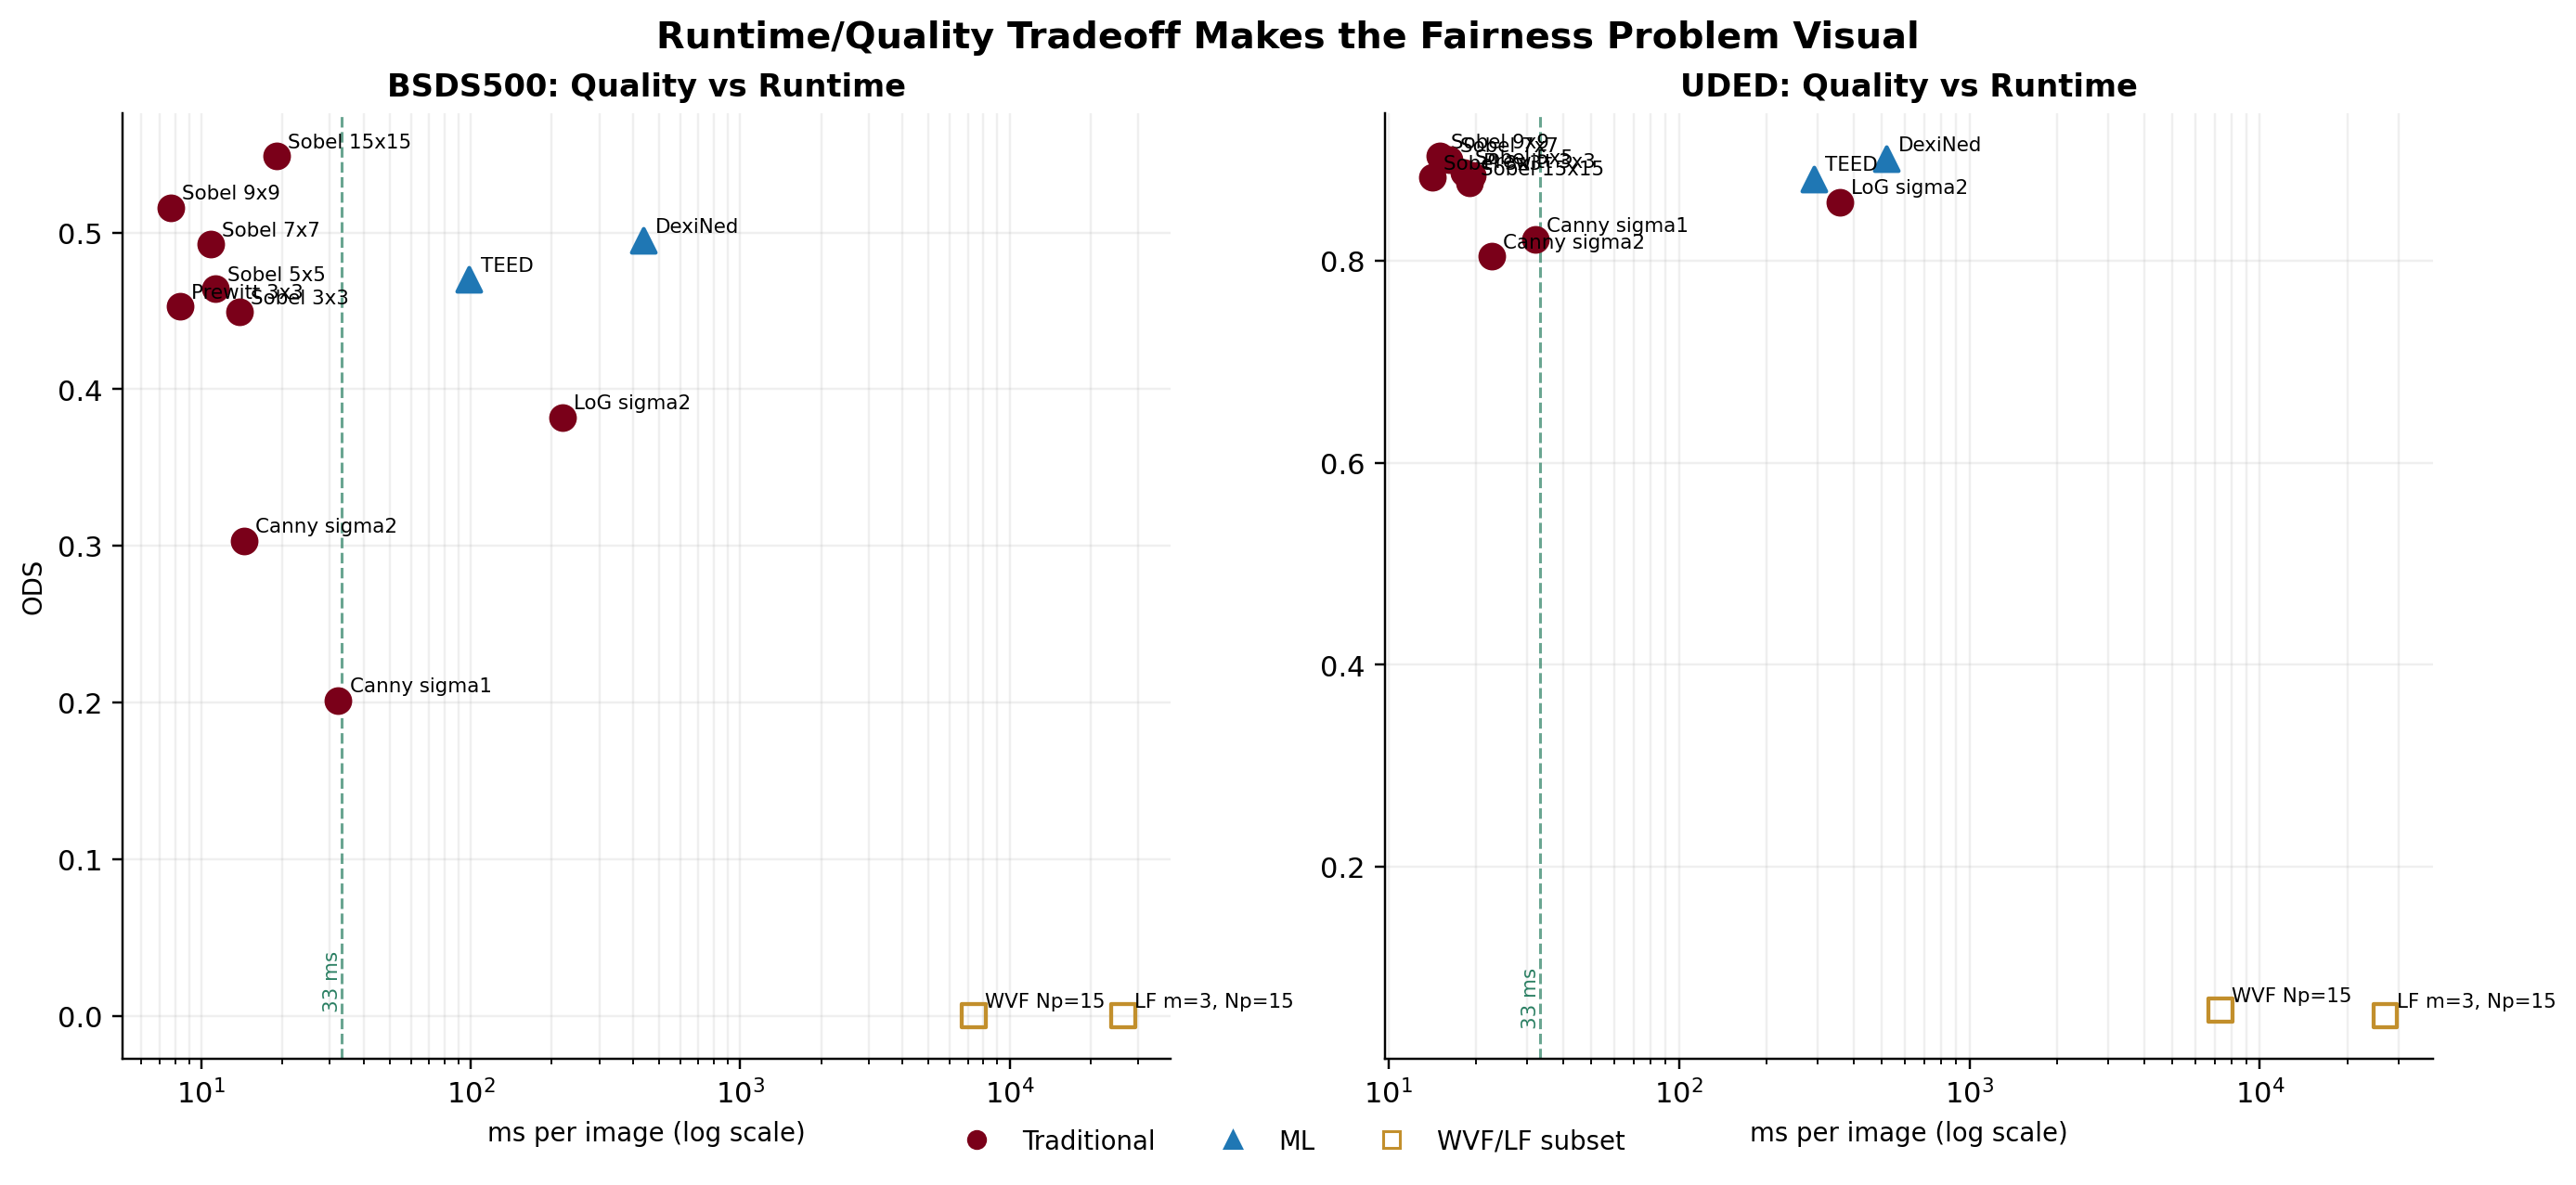
\includegraphics[width=\textwidth]{runtime_tradeoff.png}
\caption{Runtime/quality tradeoff from the repository's benchmark figures. The point of the plot is not that every method should be judged on the same clock cycle, but that the evaluation should state when CPU classical filters, CPU WVF/LF, and GPU ML baselines are being compared under different execution paths.}
\label{fig:tradeoff}
\end{figure*}

\section{What Parallelization Changes}
The new 112-core defq jobs are useful, but only in the narrow sense that they reduce the time needed to finish a sweep grid. The current full-node WVF/LF runs dispatch 200 tasks across 112 worker processes. The angle sweep dispatches 15 tasks across 15 workers. That is the correct way to use a big CPU node for independent experiments, and it is a clear improvement over the earlier serial workflow.

What it does \emph{not} do is make WVF/LF cheap. The wall-clock speedup comes from dividing a workload into many independent jobs, not from making any single WVF or LF evaluation faster. The inner kernels remain serial and costly, so a large parameter grid still takes a long time whenever one task is expensive. In that sense, the defq parallelization is an experiment-management improvement, not an algorithmic breakthrough.

The official NumPy docs are relevant here because they clarify a subtle point: NumPy itself is usually single-threaded during function calls, but linear algebra may use a BLAS backend whose threading can be controlled with environment variables such as \texttt{OMP\_NUM\_THREADS} \cite{numpyglobal}. That is exactly why the sweep scripts pin BLAS threads to one and move concurrency to the process level. This avoids oversubscription, but it also makes the bottleneck visible. If a worker is spending seconds or minutes inside a nested least-squares loop, more workers only help until the available tasks are exhausted.

\begin{table}[t]
\centering
\caption{Provisional WVF/LF Scale Evidence}
\label{tab:scale}
\scriptsize
\begin{tabular}{lccc}
\toprule
Configuration & Dataset & ODS & Time (s/img) \\
\midrule
WVF $N_p=15$ & UDED & 0.0615 & 13.24 \\
LF $N_p=15, m=3$ & UDED & 0.1333 & 39.58 \\
LF $N_p=50, m=14$ & UDED & 0.2000 & 53.84 \\
WVF $N_p=50$ & UDED & 0.0537 & 2965.91 \\
WVF $N_p=100$ & UDED & 0.0562 & 1436.21 \\
WVF $N_p=150$ & UDED & 0.0602 & 851.87 \\
WVF $N_p=15$ & BSDS500 & 0.0000 & 10.28 \\
WVF $N_p=50$ & BSDS500 & 0.0000 & 1990.91 \\
\bottomrule
\end{tabular}
\end{table}

Table~\ref{tab:scale} is provisional because the full-node scale sweeps are still running, but the serial logs already make the point that matters for practicality. Larger $N_p$ values do not produce a clean cost-benefit curve. Some LF settings improve quality on a tiny UDED subset, but the associated runtime remains high. WVF, in contrast, becomes dramatically expensive at larger $N_p$ without producing a convincing quality jump. On BSDS500, the logged WVF/LF configurations do not yet show any meaningful quality rescue.

\section{Angle Sensitivity}
The angle sweep is important because the source papers use spline-based angle estimation to argue that orientation accuracy improves. The repository's completed sweep is mixed rather than uniformly favorable. Some settings do improve over Sobel arctan, but the effect is parameter-sensitive. For example, \texttt{N\_p=50}, \texttt{36} orientations, and \texttt{SNR=2.0} reduce mean angular error from 12.35 degrees to 8.11 degrees. At other settings, especially \texttt{N\_p=15}, the spline estimate is worse than Sobel, and at \texttt{N\_p=250} the runtime becomes substantial enough to matter on its own.

The practical reading is not that spline estimation is useless. It is that the claimed advantage is neither monotonic nor free. A method that occasionally improves orientation but is expensive to run and sensitive to parameter choice is not operationally light by default. It may still be scientifically valuable, but the implementation has to earn that status.

\section{Practical Judgment}
The practical judgment from the current evidence is straightforward. WVF/LF is not yet an operationally light baseline for three separate reasons.

First, the core implementation is CPU-only and written as nested Python/NumPy loops. Second, the current parallelization only attacks experiment throughput; it does not change the per-image kernel cost. Third, the exact benchmark results on A100 do not provide a competing GPU-backed WVF/LF reference point, so the method cannot be claimed to be efficient on the same device class that accelerates the ML baselines. The repository can now run more experiments in less wall-clock time, but it still cannot make the underlying algorithm behave like a cheap filter.

This is the right place to be precise about inference. The conclusion that WVF/LF is expensive is supported directly by the code structure and the serial scale logs. The conclusion that the method is ``too slow'' in an absolute sense is more contextual and depends on what one considers an acceptable budget. But the claim that the current implementation is lightweight is not supported. The evidence points the other way.

\section{Limitations and Next Steps}
The biggest limitation of this paper is the same limitation that constrains the broader reproduction effort: the repository still does not contain BIPED, the four-image aquatic benchmark from the conference papers, or a GPU-backed WVF/LF implementation. That means the current paper can document compute realism well, but it cannot close the loop on every source-paper claim.

The most defensible next experiment is to finish the current full-node WVF/LF scale sweep and publish the result as a sensitivity study rather than as a victory lap. If larger $N_p$ and wider LF support improve quality enough to offset the runtime blow-up, then the practical conclusion should narrow. If they do not, then the critique is strengthened. Either outcome is useful, but the experiment has to be finished before the claim can be sharpened.

A second useful experiment is a true matched-support comparison. Large-support Sobel and LoG already show that ``traditional'' does not mean ``weak''; the same fairness logic should be applied wherever WVF/LF is compared to narrow-support derivatives. The authors' strongest practical claim depends on those comparisons being fair, not just favorable.

The final experiment is the one that would settle the core implementation question: a GPU or low-level CPU rewrite of WVF/LF itself. If the method can be vectorized, JIT-compiled, or ported to a proper kernel and then benchmarked fairly against the current exact A100 runs, its practical status could change. Until then, the current version should be described as computationally interesting but operationally heavy.

\section{Conclusion}
The current repository supports a narrow but useful conclusion. WVF/LF is a mathematically plausible orientation-aware formulation, and the source papers were right to explore it. But the implementation we can inspect today is a CPU-only NumPy/SciPy solver with expensive inner loops, and the new 112-core defq parallelization only makes the sweeps finish sooner. It does not make the kernel light.

The exact A100 benchmarks strengthen that conclusion indirectly. Large-support Sobel still competes well with the reproduced ML baselines on BSDS500 and UDED under an explicit 1001-threshold protocol, so the practical baseline question is not trivial. The angle sweep is mixed, which means the spline story is parameter-sensitive rather than universally decisive. The scale sweep remains the strongest unresolved question, but the early serial evidence already suggests that larger $N_p$ values can be computationally punishing.

The right characterization is therefore conservative. WVF/LF is worth studying, but the current implementation is not yet an operationally light filter. Any paper that wants to claim otherwise needs a faster kernel, a fair runtime protocol, and a completed scale study.

\begin{thebibliography}{99}

\bibitem{bagan2023thesis}
L.~Bagan, ``Wide view and line filter for enhanced image gradient computation and edge determination,'' M.S.\ thesis, Univ.\ South Carolina, 2023.

\bibitem{bagan2024oceans}
L.~Bagan and Y.~Wang, ``Wide view and line filter for enhanced gradient computation in aquatic environment,'' in \textit{Proc.\ IEEE OCEANS}, 2024.

\bibitem{bagan2025oceans}
L.~Bagan and Y.~Wang, ``Multi-scale and multi-domain edge determination with accurate gradient orientation computation in aquatic environment,'' in \textit{Proc.\ IEEE OCEANS}, 2025.

\bibitem{torchcuda}
PyTorch, \texttt{torch.cuda.is\_available}, official documentation. [Online]. Available: \url{https://docs.pytorch.org/docs/stable/generated/torch.cuda.is_available}. Accessed: 2026-03-28.

\bibitem{torchcudans}
PyTorch, \texttt{torch.cuda}, official documentation. [Online]. Available: \url{https://docs.pytorch.org/docs/stable/cuda.html}. Accessed: 2026-03-28.

\bibitem{numpyglobal}
NumPy, ``Global State,'' official documentation. [Online]. Available: \url{https://numpy.org/doc/1.21/reference/global_state.html}. Accessed: 2026-03-28.

\bibitem{slurmsbatch}
SchedMD, ``sbatch,'' official Slurm documentation. [Online]. Available: \url{https://slurm.schedmd.com/sbatch.html}. Accessed: 2026-03-28.

\end{thebibliography}

\end{document}
